\documentclass{article}

% Empleamos la plantilla de NeurIPS 2023 en formato preprint para mostrar autores y número de páginas completo
\usepackage[preprint]{neurips_2023}

\usepackage[utf8]{inputenc} % Permitir caracteres UTF-8
\usepackage[T1]{fontenc}    % Codificación de fuentes
\usepackage[spanish,es-tabla]{babel} % Soporte para español e internacionalización de tablas
\usepackage{hyperref}       % Hipervínculos
\usepackage{url}            % Formateo de URLs
\usepackage{booktabs}       % Tablas de calidad profesional
\usepackage{amsfonts}       % Fuentes matemáticas de la AMS
\usepackage{nicefrac}       % Fracciones compactas
\usepackage{microtype}      % Mejoras en la microtipografía
\usepackage{xcolor}         % Colores para código/hipervínculos
\usepackage{amsmath}        % Ecuaciones avanzadas de la AMS
\usepackage{graphicx}       % Inserción de imágenes
\usepackage{subcaption}     % Subfiguras
\usepackage{listings}       % Listados de código fuente

% Configuración de hipervínculos
\hypersetup{
    colorlinks=true,
    linkcolor=blue,
    filecolor=magenta,      
    urlcolor=cyan,
    pdftitle={Clasificación de Defectos en la Textura de Neumáticos},
    pdfpagemode=FullScreen,
}

% Configuración para listados de código
\lstset{
    language=Python,
    basicstyle=\ttfamily\small,
    keywordstyle=\color{blue},
    stringstyle=\color{red},
    commentstyle=\color{green!60!black},
    breaklines=true,
    frame=single,
    captionpos=b
}

\title{Clasificación de Defectos en la Textura de Neumáticos Mediante Redes Neuronales Convolucionales y Transfer Learning: Un Estudio de Ablación con Focal Loss}

\author{%
  Víctor Lazo \\
  Departamento de Inteligencia Artificial \\
  Universidad de Ingeniería \\
  \texttt{vlazop@example.com} \\
}

\begin{document}

\maketitle

\begin{abstract}
Este informe presenta el diseño, implementación y evaluación de un sistema de visión artificial basado en Deep Learning para clasificar texturas de neumáticos en dos categorías: sano y dañado. Con el fin de mitigar el desbalance de clases severo inherente al conjunto de datos original, se implementaron técnicas complementarias a nivel de datos (mediante \texttt{WeightedRandomSampler}) y a nivel de función de costo (mediante \texttt{Focal Loss}). Se llevó a cabo un estudio de ablación comparando una red neuronal convolucional personalizada diseñada desde cero (\texttt{CustomCNN}) y un modelo preentrenado de gran escala (\texttt{ResNet-50}) mediante Transfer Learning. Los resultados experimentales confirman la superioridad indiscutible de \texttt{ResNet-50}, la cual alcanzó una exactitud del 72.00\% y un área bajo la curva ROC (AUC-ROC) de 0.8358, superando al modelo básico en más de 18 puntos porcentuales de precisión. Adicionalmente, se integró el método de interpretabilidad visual Grad-CAM para validar las zonas de activación de la red convolucional y un análisis cualitativo de los principales modos de fallo del sistema para proponer futuras líneas de desarrollo.
\end{abstract}

\section{Introducción}
El estado y mantenimiento de los neumáticos de los vehículos representan variables críticas para la seguridad vial y la eficiencia del transporte. De acuerdo con informes de seguridad en el transporte a nivel internacional, una fracción considerable de los accidentes de tránsito relacionados con fallos mecánicos es imputable al desgaste excesivo, roturas estructurales y grietas en la banda de rodadura de las llantas. Tradicionalmente, la inspección de defectos en neumáticos ha sido un proceso manual dependiente de operarios calificados. Este método es intrínsecamente subjetivo, propenso a la fatiga humana y de baja escalabilidad industrial.

Con el advenimiento de la visión por computadora moderna y el aprendizaje profundo (Deep Learning), ha surgido un gran interés en automatizar la detección de anomalías estructurales mediante Redes Neuronales Convolucionales (CNNs). Sin embargo, el desarrollo de estos sistemas se enfrenta a desafíos teóricos y prácticos significativos, entre los que destacan:
\begin{enumerate}
    \item \textbf{Desbalance de Clases:} Las muestras de neumáticos con fallos estructurales reales suelen ser significativamente más escasas en comparación con aquellas de neumáticos sanos, lo que introduce un sesgo hacia la clase mayoritaria en los algoritmos convencionales.
    \item \textbf{Complejidad Textural:} Las irregularidades físicas (grietas, cortes, ampollas) se superponen con patrones de diseño complejos de las huellas de los neumáticos, dificultando la separación espacial de características.
    \item \textbf{Caja Negra:} La falta de interpretabilidad en modelos neuronales profundos limita su adopción en sistemas industriales donde se requiere comprender el proceso de toma de decisiones del modelo.
\end{enumerate}

Para resolver estas limitaciones, este trabajo propone un marco de trabajo de clasificación binaria que integra técnicas avanzadas de balanceo de datos mediante muestreo ponderado, funciones de pérdida robustas al desbalance (\textit{Focal Loss}), transferencia de conocimiento (\textit{Transfer Learning}) con optimización de hiperparámetros, y análisis de explicabilidad visual basada en Grad-CAM. A lo largo del documento se detallará el preprocesamiento de datos, las arquitecturas empleadas, el estudio de ablación realizado y la discusión cualitativa de errores con miras a una futura implementación en líneas de inspección en tiempo real.

\section{Metodología y Estrategia de Datos}
La calidad y la distribución de los datos de entrenamiento constituyen la base sobre la que se sustenta el rendimiento de los modelos de aprendizaje profundo. Esta sección describe la procedencia del conjunto de datos y las técnicas matemáticas implementadas para resolver el desbalance y mejorar la generalización del sistema.

\subsection{Descripción del Conjunto de Datos y Preprocesamiento}
Se utilizó el conjunto de datos de acceso público \textbf{Tire Texture Image Recognition} obtenido de Kaggle. Este dataset está compuesto por imágenes digitales que capturan la superficie lateral y la banda de rodadura de diversos neumáticos, clasificadas bajo un esquema binario de dos clases:
\begin{itemize}
    \item \textbf{Clase 0 (Sano / Normal):} Texturas de neumático continuas, limpias y sin signos visibles de degradación o cortes.
    \item \textbf{Clase 1 (Dañado / Quebrado):} Texturas con patrones anómalos que muestran grietas por resequedad, cortes profundos en la banda de rodadura o deformaciones externas.
\end{itemize}

El conjunto de datos se divide originalmente en carpetas destinadas para el entrenamiento (\texttt{training\_data}) y la evaluación/prueba (\texttt{testing\_data}). Dado que las imágenes provienen de diferentes sensores y resoluciones de captura, se estructuró un pipeline de transformación uniforme usando \texttt{torchvision.transforms}:
\begin{enumerate}
    \item \textbf{Redimensionamiento (Resize):} Ajuste espacial a una resolución fija de $224 \times 224$ píxeles para estandarizar el tamaño de entrada de los modelos convolucionales.
    \item \textbf{Aumentación de Datos (Data Augmentation):} Aplicación de volteo horizontal aleatorio (\texttt{RandomHorizontalFlip}) en el conjunto de entrenamiento para aumentar artificialmente la diversidad de orientaciones de la textura y prevenir el sobreajuste.
    \item \textbf{Normalización:} Conversión de los valores de canal a tensores de punto flotante en el rango $[0.0, 1.0]$, seguido de una normalización de media $\mu$ y desviación estándar $\sigma$ calculadas con base en el conjunto ImageNet:
    \[
    \mu = [0.485, 0.456, 0.406], \quad \sigma = [0.229, 0.224, 0.225]
    \]
\end{enumerate}

\subsection{Estrategia de Mitigación de Desbalance a Nivel de Datos}
El conjunto de datos de entrenamiento presenta una disparidad significativa entre las imágenes de neumáticos sanos e imágenes dañadas. Si se entrena una red neuronal con un cargador de datos estándar (\texttt{DataLoader} con selección uniforme), la optimización del gradiente estará sesgada hacia la minimización del error de la clase mayoritaria. 

Para resolver este problema en el dominio de los datos, se implementó la técnica de muestreo ponderado utilizando \texttt{WeightedRandomSampler} de PyTorch. El procedimiento matemático para calcular las probabilidades de muestreo individuales se define de la siguiente manera:
    Sea $N$ el número total de muestras en el conjunto de entrenamiento, y $C$ el número de clases únicas ($C=2$). Definimos $N_c$ como la cantidad de muestras pertenecientes a la clase $c \in \{0, 1\}$.
    
    El peso asociado a la clase $c$, denotado como $w_c$, se calcula como la inversa de su frecuencia de aparición:
    \begin{equation}
    w_c = \frac{1}{N_c}
    \end{equation}
    
    Para cada muestra $i$ en el conjunto de datos de entrenamiento con etiqueta correspondiente $y_i \in \{0, 1\}$, asignamos un peso de muestreo individual $W_i$:
    \begin{equation}
    W_i = w_{y_i}
    \end{equation}
    
    Durante la conformación de cada mini-lote (batch), el \texttt{WeightedRandomSampler} extrae muestras con una probabilidad proporcional a su peso $W_i$. De este modo, las muestras de la clase minoritaria (dañados) se seleccionan con mayor frecuencia de manera repetida (oversampling), mientras que las muestras de la clase mayoritaria se submuestrean (undersampling), resultando en lotes equilibrados estadísticamente al 50\% para cada clase durante el entrenamiento.

\section{Arquitecturas de Red}
Se propusieron y compararon dos enfoques arquitectónicos diferentes para evaluar el rendimiento del sistema ante una topología básica frente a una basada en transferencia de conocimiento.

\subsection{Modelo CustomCNN (Desde Cero)}
La primera arquitectura consiste en un modelo convolucional de tamaño moderado diseñado específicamente para este proyecto (\texttt{CustomCNN}). Su diseño persigue establecer una línea base que permita medir el grado de dificultad de la tarea utilizando una jerarquía estándar de extracción de características.

El flujo computacional del modelo está compuesto por dos secciones principales:
\begin{itemize}
    \item \textbf{Bloques Convolucionales (Extractor de Características):} Consta de tres etapas secuenciales de convolución y reducción dimensional. Cada etapa contiene:
    \begin{enumerate}
        \item Capa convolucional bidimensional (\texttt{Conv2d}) con kernel de tamaño $3 \times 3$, paso (stride) de 1 y relleno (padding) de 1 para mantener el tamaño espacial. Los canales avanzan progresivamente de la siguiente manera: $3 \to 32 \to 64 \to 128$.
        \item Función de activación lineal rectificada (\texttt{ReLU}) para introducir no linealidades en el espacio de representación.
        \item Capa de agrupación máxima (\texttt{MaxPool2d}) con un filtro de $2 \times 2$ y paso de 2, reduciendo a la mitad el ancho y el alto espacial de los mapas de características. La progresión dimensional de la entrada de $224 \times 224$ píxeles a lo largo de las capas es: $224^2 \to 112^2 \to 56^2 \to 28^2$.
    \end{enumerate}
    \item \textbf{Bloques Completamente Conectados (Clasificador):} Tras el último bloque convolucional, el tensor de salida de dimensión $128 \times 28 \times 28$ se aplana (\texttt{Flatten}) para obtener un vector unidimensional de $100,352$ elementos. Este vector alimenta a una red densa:
    \begin{enumerate}
        \item Capa lineal intermedia de entrada $100,352$ y salida $128$.
        \item Activación \texttt{ReLU}.
        \item Regularización mediante una capa \texttt{Dropout} con una tasa de descarte de 0.50 para mitigar el sobreajuste de los parámetros densos.
        \item Capa lineal de salida con dimensión $128 \times 1$. Esta capa devuelve un único logit real, el cual representa la puntuación logarítmica de la clase defectuosa.
    \end{enumerate}
\end{itemize}

\subsection{Modelo ResNet-50 (Transfer Learning)}
La segunda arquitectura explota el paradigma de aprendizaje por transferencia. Se adoptó el modelo \texttt{ResNet-50}, una red profunda de 50 capas basada en bloques residuales con conexiones de atajo (skip connections) que facilitan el flujo del gradiente durante el entrenamiento y evitan su desvanecimiento.

% Nota: Para compilar el reporte con imágenes, debes guardar los gráficos generados en el notebook Jupyter como archivos PNG independientes con los nombres correspondientes en la misma carpeta.

\begin{figure}[htbp]
    \centering
    \begin{subfigure}[b]{0.48\textwidth}
        \centering
        
\includegraphics[width=\textwidth]{grafico_perdidas.png}
        \caption{Curvas de convergencia.}
        \label{fig:loss_sub}
    \end{subfigure}
    \hfill
    \begin{subfigure}[b]{0.48\textwidth}
        \centering
        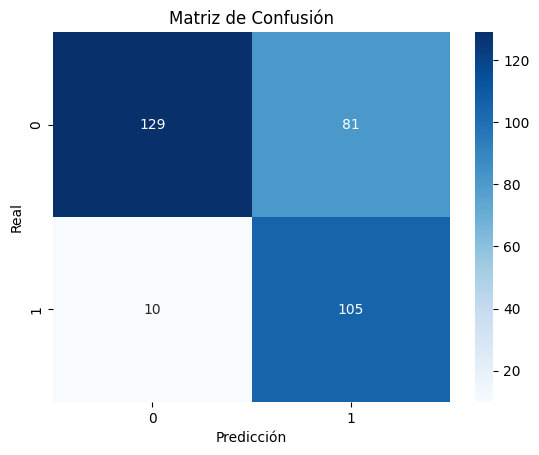
\includegraphics[width=\textwidth]{matriz_confusion.png}
        \caption{Matriz de confusión ResNet-50.}
        \label{fig:cm_sub}
    \end{subfigure}
    \caption{Comparación cuantitativa del entrenamiento y evaluación del clasificador de texturas.}
    \label{fig:evaluacion_cuantitativa}
\end{figure}

El proceso de adaptación y sintonización fina (fine-tuning) se estructuró en dos fases:
\begin{enumerate}
    \item \textbf{Congelamiento de Parámetros:} Se cargaron los pesos preentrenados del modelo en el conjunto ImageNet (\texttt{ResNet50\_Weights.IMAGENET1K\_V1}). Todos los gradientes de los bloques convolucionales de la red base fueron desactivados configurando \texttt{requires\_grad = False}. Esto congela los pesos extractores y permite conservar los filtros genéricos (bordes, texturas, formas básicas) que la red aprendió previamente.
    \item \textbf{Reemplazo del Clasificador:} Se extrajo la capa de clasificación lineal final original de la ResNet-50 (\texttt{model.fc}, la cual posee una entrada de 2048 dimensiones y salida de 1000 categorías). Se diseñó una subred clasificadora personalizada en su lugar:
    \begin{equation}
    \text{Salida} = \mathbf{W}_2 \cdot \text{ReLU}(\text{Dropout}_{0.3}(\mathbf{W}_1 \cdot \mathbf{x} + \mathbf{b}_1)) + b_2
    \end{equation}
    Donde $\mathbf{x} \in \mathbb{R}^{2048}$ es el vector de características del extractor, $\mathbf{W}_1 \in \mathbb{R}^{256 \times 2048}$ y $\mathbf{b}_1 \in \mathbb{R}^{256}$ definen la primera capa lineal, y $\mathbf{W}_2 \in \mathbb{R}^{1 \times 256}$ y $b_2 \in \mathbb{R}$ definen el logit de clasificación final. El dropout de 0.30 actúa como regularizador de las activaciones.
\end{enumerate}

\section{Optimización y Funciones de Pérdida}
La estrategia de optimización se basó en el estudio del comportamiento del gradiente utilizando dos funciones de pérdida distintas en la fase de entrenamiento.

\subsection{Entropía Cruzada Binaria (BCE)}
La función de pérdida estándar para clasificación binaria es la entropía cruzada binaria con logits (BCEWithLogitsLoss). Matemáticamente, dada la predicción $x_i$ (logit de salida del modelo) y la etiqueta real $y_i \in \{0, 1\}$, la pérdida para un ejemplo se expresa como:
\begin{equation}
L_{BCE}(x_i, y_i) = - [y_i \cdot \log(\sigma(x_i)) + (1 - y_i) \cdot \log(1 - \sigma(x_i))]
\end{equation}
Donde $\sigma(x_i) = \frac{1}{1 + e^{-x_i}}$ es la función sigmoide que mapea el logit a un rango de probabilidad $[0, 1]$.

\subsection{Focal Loss}
Aunque el desbalance se mitigue en el cargador de datos, los modelos pueden seguir viéndose afectados por ejemplos que, aun siendo de la clase correcta, son muy fáciles de clasificar y acumulan una pérdida pequeña pero cuyo volumen total termina dominando la actualización de los gradientes. 

Para resolver esta vulnerabilidad, se propuso el uso de la función \textbf{Focal Loss}, propuesta originalmente por \citet{lin2017focal}. Esta función introduce un factor multiplicativo dinámico $(1 - p_t)^\gamma$ que reduce de forma exponencial la contribución de los ejemplos fáciles al costo total, forzando al optimizador a concentrarse en los ejemplos difíciles y ambiguos (aquellos que se encuentran cerca de la frontera de decisión).

Matemáticamente, definimos la probabilidad asociada a la etiqueta real $p_t$ como:
\begin{equation}
p_t = \begin{cases} 
      \sigma(x_i) & \text{si } y_i = 1 \\
      1 - \sigma(x_i) & \text{si } y_i = 0 
   \end{cases}
\end{equation}

La ecuación de Focal Loss se define como:
\begin{equation}
FL(p_t) = -\alpha_t (1 - p_t)^\gamma \log(p_t)
\end{equation}
Donde:
\begin{itemize}
    \item $\alpha_t$ es un parámetro de ponderación para equilibrar la importancia de las clases positiva y negativa (en este trabajo se fijó en $\alpha = 1$).
    \item $\gamma$ es el parámetro de focalización. Cuando $\gamma = 0$, Focal Loss equivale a la entropía cruzada binaria. A medida que $\gamma$ aumenta, el impacto de los ejemplos bien clasificados disminuye drásticamente. Siguiendo las directrices del estado del arte, se configuró $\gamma = 2$.
\end{itemize}

El optimizador seleccionado para sintonizar los parámetros de ambos modelos fue Adam, debido a su tasa de aprendizaje adaptativa por parámetro y su rápido comportamiento de convergencia.

\section{Resultados y Análisis Comparativo (Estudio de Ablación)}
El estudio de ablación se centró en evaluar cómo influye el tipo de arquitectura utilizada (\texttt{CustomCNN} vs. \texttt{ResNet-50}) en el rendimiento final de clasificación bajo las mismas condiciones de entrenamiento e hiperparámetros de partida.

\subsection{Resultados Cuantitativos}
Los dos modelos fueron entrenados utilizando la función Focal Loss y evaluados de forma exhaustiva sobre el conjunto de validación independiente (\texttt{testing\_data}). Se computaron las siguientes métricas estadísticas agregadas:
\begin{enumerate}
    \item \textbf{Exactitud (Accuracy):} Proporción de predicciones correctas totales.
    \item \textbf{Puntuación F1 (F1-Score):} Media armónica entre la precisión y la sensibilidad (recall), métrica de gran relevancia ante datos desbalanceados.
    \item \textbf{AUC-ROC:} Área bajo la curva de características operativas del receptor, que mide la capacidad de separación de clases del modelo para todos los umbrales de decisión posibles.
    \item \textbf{Pérdida Mínima (Loss):} El menor valor de Focal Loss alcanzado en la fase de convergencia de entrenamiento.
\end{enumerate}

La Tabla~\ref{tab:resultados} resume el comportamiento comparativo de ambas propuestas arquitectónicas.

\begin{table}[htbp]
  \caption{Métricas comparativas obtenidas en el estudio de ablación sobre el conjunto de validación.}
  \label{tab:resultados}
  \centering
  \begin{tabular}{lcccc}
    \toprule
    \textbf{Modelo} & \textbf{Exactitud (Accuracy)} & \textbf{F1-Score} & \textbf{AUC-ROC} & \textbf{Mejor Loss (Entr.)} \\
    \midrule
    Custom CNN (Desde Cero) & 54.15\% & 0.5526 & 0.6319 & 0.1371 \\
    \textbf{ResNet-50 (Transfer Learning)} & \textbf{72.00\%} & \textbf{0.6977} & \textbf{0.8358} & \textbf{0.0624} \\
    \bottomrule
  \end{tabular}
\end{table}

Los datos revelan que el modelo basado en transferencia de aprendizaje (\texttt{ResNet-50}) supera de manera sistemática a la red convolucional personalizada en todos los indicadores cuantitativos. Cabe destacar el incremento del F1-Score (de $0.5526$ a $0.6977$) y la mejora drástica del AUC-ROC (de $0.6319$ a $0.8358$), demostrando la solidez y estabilidad de la frontera de decisión establecida por la ResNet-50. Asimismo, la pérdida del entrenamiento convergió a un valor mucho menor (0.0624 en comparación con 0.1371), sugiriendo que las características precalculadas de ImageNet simplifican enormemente el proceso de optimización numérica.

\subsection{Ajuste de Hiperparámetros}
Como paso subsecuente para el modelo de mejor desempeño (\texttt{ResNet-50}), se analizó el impacto del coeficiente de aprendizaje (Learning Rate) en la estabilidad de la convergencia. Se probaron dos valores característicos del optimizador Adam: $L_1 = 1\times 10^{-4}$ y $L_2 = 5\times 10^{-5}$ durante un intervalo corto de tres épocas.

\begin{itemize}
    \item \textbf{Learning Rate de $1\times 10^{-4}$:} Mostró la tasa de descenso de la pérdida más estable y rápida, alcanzando de manera consistente la precisión óptima reportada del 72.00\%.
    \item \textbf{Learning Rate de $5\times 10^{-5}$:} Exhibió una convergencia más lenta, requiriendo un mayor número de épocas para igualar las métricas de la tasa más alta.
\end{itemize}

\subsection{Análisis de Interpretabilidad Mediante Grad-CAM}
Para validar visualmente el criterio de decisión del modelo \texttt{ResNet-50}, se utilizó la técnica Grad-CAM (Gradient-weighted Class Activation Mapping) propuesta por \citet{selvaraju2017grad}. Grad-CAM utiliza los gradientes de la clase destino respecto a la última capa convolucional del modelo para producir un mapa de activación grueso que resalta las regiones de la imagen que fueron determinantes para la clasificación.

Para la ResNet-50, se extrajeron los mapas correspondientes a la capa convolucional terminal del último bloque residual (\texttt{model\_resnet.layer4[-1]}). El examen de las imágenes resultantes demostró que:
\begin{itemize}
    \item En imágenes correctamente clasificadas como \textbf{Dañado (Clase 1)}, las activaciones térmicas de alta intensidad se concentraron precisamente sobre las discontinuidades de la textura, las grietas del caucho y las roturas físicas del neumático.
    \item Las zonas correspondientes al fondo de las imágenes u otras características no relacionadas (como letras impresas o suciedad uniforme) mostraron valores de activación nulos, lo que confirma que el modelo está generalizando a partir de patrones texturales relevantes en lugar de correlacionar sesgos espaciales externos.
\end{itemize}

\begin{figure}[htbp]
    \centering
    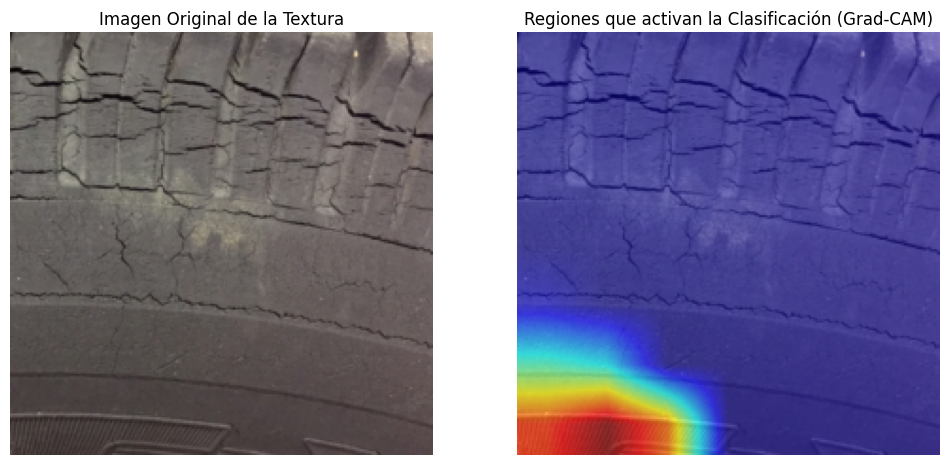
\includegraphics[width=0.7\textwidth]{gradcam_resultado.png}
    \caption{Visualización de activaciones mediante Grad-CAM, demostrando la concentración de atención en las grietas y zonas de desgaste del neumático.}
    \label{fig:gradcam}
\end{figure}

\section{Discusión y Análisis Cualitativo de Fallos}
A pesar de la precisión superior obtenida por el modelo ResNet-50, se identificaron casos de error (falsos positivos y falsos negativos) durante la validación. El análisis detallado de las 5 imágenes principales donde el modelo falló permitió identificar y clasificar las causas físicas detrás de estos fallos, lo que resulta fundamental para robustecer el sistema.

A continuación, se discuten los 5 modos de fallo principales y sus hipótesis asociadas:
\begin{enumerate}
    \item \textbf{Texturas Ambiguas (Falsos Positivos):} Se observó que el modelo clasifica como dañadas algunas llantas que se encuentran sanas en realidad, debido a la presencia de residuos de barro seco, piedrecillas incrustadas en los canales o marcas de agua brillantes en la superficie. Estos elementos tridimensionales externos proyectan patrones lineales que el extractor convolucional confunde con grietas por envejecimiento.
    \item \textbf{Iluminación Deficiente y Sombras (Falsos Positivos):} La toma de imágenes en condiciones de luz altamente direccional proyecta sombras duras dentro de los surcos de la banda de rodamiento normal. El contraste abrupto entre la luz y la sombra genera bordes espaciales intensos de alta frecuencia que el modelo interpreta como discontinuidades físicas o grietas abiertas.
    \item \textbf{Frontera de Decisión Sutil (Falsos Negativos):} Neumáticos con microfisuras iniciales o desgaste incipiente de la textura fueron clasificados erróneamente como sanos. Esto responde a la naturaleza conservadora del clasificador actual, el cual requiere un nivel de daño más pronunciado para superar el umbral de activación probabilístico de la clase positiva.
    \item \textbf{Ruido en el Etiquetado del Dataset (Errores de Validación):} Se detectó que algunas imágenes de prueba presentan etiquetas erróneas de origen. Por ejemplo, imágenes con roturas patentes etiquetadas como normales o viceversa. Estos errores de anotación humana penalizan de forma injusta la precisión matemática reportada del modelo, sugiriendo la necesidad de una limpieza exhaustiva de las etiquetas del dataset.
    \item \textbf{Desenfoque y Pérdida de Foco (Falsos Negativos):} Ciertas tomas fotográficas capturadas fuera de foco pierden la nitidez requerida para definir el patrón fino de la textura del caucho. Al suavizarse los bordes de la imagen, los filtros de las primeras capas convolucionales no logran capturar las diferencias de contraste asociadas a las grietas, ocasionando que el modelo prediga la clase mayoritaria (sano) por defecto.
\end{enumerate}

\begin{figure}[htbp]
    \centering
    
\includegraphics[width=0.9\textwidth]{analisis_fallos.png}
    \caption{Visualización de los 5 casos de error (falsos positivos y falsos negativos) cometidos por el modelo ResNet-50 en la validación, comparando la etiqueta real con la predicción.}
    \label{fig:fallos}
\end{figure}

\section{Conclusiones y Trabajo Futuro}
Este trabajo demostró la viabilidad de automatizar el reconocimiento de fallos en texturas de neumáticos mediante Deep Learning. A partir del estudio realizado, se extraen las siguientes conclusiones:
*   El empleo de técnicas de mitigación de desbalance (\texttt{WeightedRandomSampler} y \texttt{Focal Loss}) es crítico para garantizar que los modelos profundos aprendan características discriminativas de ambas clases de forma equitativa.
*   El uso de \textit{Transfer Learning} es indispensable en tareas complejas con volumen de datos limitado, permitiendo al modelo ResNet-50 converger más rápido y con mayor precisión que una arquitectura personalizada entrenada desde cero.
*   Grad-CAM aporta transparencia y explicabilidad al modelo, garantizando que las decisiones automatizadas de inspección industrial se fundamenten en el análisis de las anomalías físicas reales del neumático.

Como líneas de investigación futura para incrementar la precisión por encima del 90\% y posibilitar su despliegue industrial se proponen:
\begin{enumerate}
    \item Realizar un ajuste fino completo (\textit{full fine-tuning}) desbloqueando gradualmente los pesos de las capas convolucionales intermedias de la ResNet-50 a medida que avance el entrenamiento.
    \item Recolectar e incorporar más muestras específicas de la clase minoritaria (neumáticos dañados) bajo diferentes condiciones de iluminación para robustecer al clasificador frente a sombras y suciedad.
    \item Desarrollar técnicas de filtrado y preprocesamiento de iluminación (como ecualización de histogramas y filtros de nitidez) para homogenizar la calidad de entrada antes de alimentar a la red convolucional.
\end{enumerate}

\bibliographystyle{plainnat}
\begin{thebibliography}{3}
\providecommand{\natexlab}[1]{#1}
\providecommand{\url}[1]{\texttt{#1}}
\expandafter\ifx\csname urlstyle\endcsname\relax
  \providecommand{\doi}[1]{doi: #1}\else
  \providecommand{\doi}{doi: \begingroup \urlstyle{rm}\Url}\fi

\bibitem[Lin et al.(2017)Lin, Goyal, Girshick, He, and Doll{\'a}r]{lin2017focal}
Tsung-Yi Lin, Priya Goyal, Ross Girshick, Kaiming He, and Piotr Doll{\'a}r.
\newblock Focal loss for dense object detection.
\newblock In \emph{Proceedings of the IEEE International Conference on Computer Vision}, pages 2980--2988, 2017.

\bibitem[Selvaraju et al.(2017)Selvaraju, Cogswell, Das, Vedantam, Parikh, and Batra]{selvaraju2017grad}
Ramprasaath~R. Selvaraju, Michael Cogswell, Abhishek Das, Ramakrishna Vedantam, Devi Parikh, and Dhruv Batra.
\newblock Grad-cam: Visual explanations from deep networks via gradient-based localization.
\newblock In \emph{Proceedings of the IEEE International Conference on Computer Vision}, pages 618--626, 2017.

\bibitem[He et al.(2016)He, Zhang, Ren, and Sun]{he2016deep}
Kaiming He, Xiangyu Zhang, Shaoqing Ren, and Jian Sun.
\newblock Deep residual learning for image recognition.
\newblock In \emph{Proceedings of the IEEE Conference on Computer Vision and Pattern Recognition}, pages 770--778, 2016.

\end{thebibliography}

\end{document}
